\subsection{Structures}
\begin{frame}{Obtaining the Protein}
\begin{columns}
\column{0.7\textwidth}
There are many repositorys for protein crystal structures:
\begin{itemize}
	\item \href{https://www.rcsb.org/}{https://www.rcsb.org/}
	\item \href{https://www.uniprot.org/}{https://www.uniprot.org/}
	\item \href{https://www.wwpdb.org/}{https://www.wwpdb.org/}
\end{itemize}\vspace{1cm}

Our protein has the PDB code 1N23:
\href{https://www.rcsb.org/structure/1N23}{https://www.rcsb.org/structure/1N23}
\column{0.3\textwidth}
\begin{figure}
\includegraphics[width=0.95\textwidth]{figures/System/1n23Render.png}
\end{figure}
\end{columns}
\end{frame}

\begin{frame}{Obtaining the Ligand}
\begin{columns}
\column{0.5\textwidth}
\begin{figure}
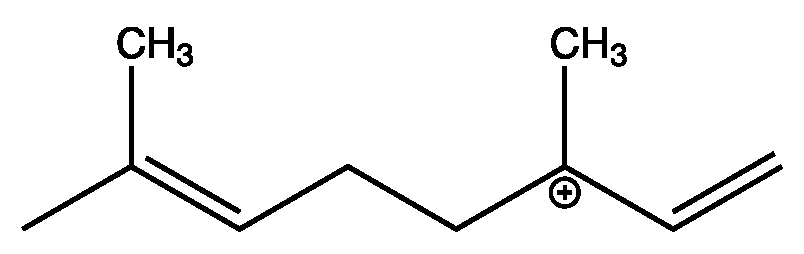
\includegraphics[width=0.6\textwidth]{../Graphics/1n20Lig.eps}
\end{figure}
\begin{itemize}
\item Structure 1 from the reaction pathway
\item Other intermediates from this reaction scheme should also work
\end{itemize}\vspace{1cm}

{\tiny
M.Weitman, D. Major, Challenges Posed to Bornyl Diphosphate Synthase: Diverging Reaction Mechanisms in Monoterpenes,  J. Am. Chem. Soc., 2010, \textbf{132} (18), 6349-6360}
\column{0.5\textwidth}
\begin{figure}
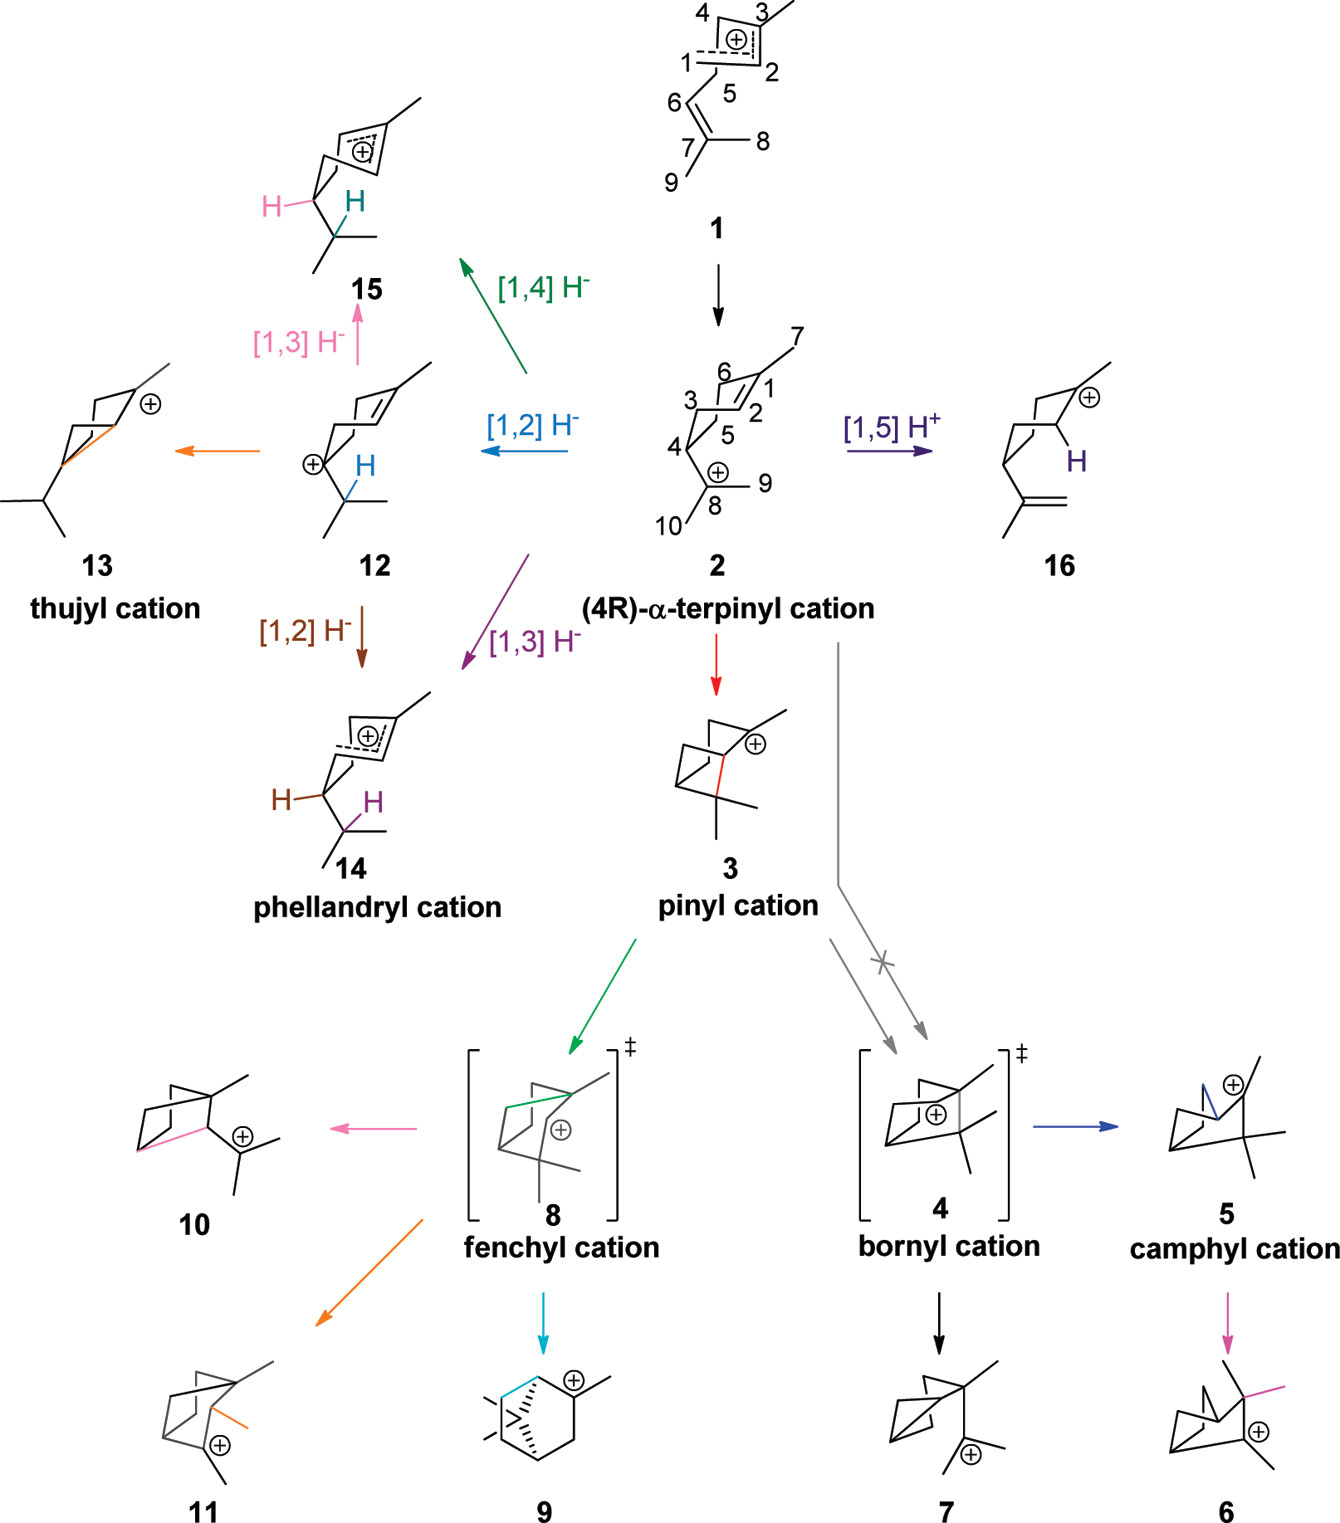
\includegraphics[height=0.7\textheight]{figures/System/RXNScheme.jpeg}
\end{figure}
\end{columns}
\end{frame}